\documentclass{article}
\usepackage{graphicx}
\usepackage[utf8]{inputenc}
\usepackage[english]{babel}
\usepackage{url}
\usepackage{indentfirst}
\usepackage{hyperref}


\begin{document}
\begin{titlepage}
 
	\begin{center}
		\begin{LARGE}
			Vysoké Učení Technické \\
			\vspace{0.7cm}
		\end{LARGE}
		\vspace{2cm}
        
		
\includegraphics[scale=1]{FIT_zkracene_barevne_PANTONE_CZ.eps}

	\end{center}	
	
	\vfill
	\vspace{2cm}
	
	\begin{center}
		\begin{Large}
			Dokumentace pro projekt k předmětu IMS \\
		\end{Large}
		\bigskip
		\begin{Huge}
			 Model studentské menzy\\
		\end{Huge}
	\end{center}
 
	\vfill
 
	\begin{center}
		\begin{Large}
			\today
		\end{Large}
	\end{center}
 
	\vfill
 
	\begin{flushleft}
		\begin{large}
			\begin{tabular}{llllll}
				Autoři:
                	& Peter Malina, 	& \url{xmalin26@stud.fit.vutbr.cz} & & \\
                	& Vojtech Mašek,	& \url{xmasek15@stud.fit.vutbr.cz} & & \\
			\end{tabular}
		\end{large}
	\end{flushleft}
\end{titlepage}

\tableofcontents
\newpage
	
\section{Úvod}
Táto dokumentácia popisuje simuláciu \cite[str. 8]{ims} školskej menzy FIT VUT v Brne, presnejšie menzy Starý Pivovar. Počet študentov vstupujúcich do menzy sa v čase líši, preto je táto práca zameraná práve na simulácie v rôznych časoch od otvorenia. Experimenty sa snažia určiť časti systému menzy, vďaka ktorým jej chod nie je plynulý v daných časových úsekochý. Simulácia rieši hlavné činnosti menzy, preto nie je úplne podrobná, no využíva priemery nameraných hodnôt, vďaka ktorým by aj pod-činnosti mali byť zahrnuté.

Za účelom správneho vytvorenia modelu \cite[str. 7]{ims} boli vykonané dve hodinové merania a použité dostupné informácie o menzách \cite{menzy}

\subsection{Autori a zdroje faktov}
Autormi práce sú Peter Malina a Vojtech Mašek.

Vstupné dáta modelu boli vytvorené na základe pozorovaní v menze a kozultovaní s jej zákazníkmi. Na hodnotách sa teda môže prejaviť odchylka spôsobená vybratou vzorkou ľudí.

\subsection{Validita projektu}
Overenie validity modelu \cite[str. 37]{ims} bolo dokázané porovnaním výsledného chovania modelu \cite[str. 24]{ims} a systému \cite[str. 7]{ims} ktorý bol vymodelovaný.

Počet študentov prichádzajúcich do menzy bol overený na základe priameho pozorovania príchodov v rámci niekoľko-násobného pozorovania v rôznych časových úsekoch. Pozorovania boli rozdelené do štyroch úsekov: čas po otvorení menzy, v špičke, mimo špičky a pred zatvorením. Tieto časy boli spriemerované pre celkovú simuláciu. Stredná hodnota funkcie exponenciálnej pravdepodobnosti \cite[str. 91]{ims} je 17.5 sekundy. Táto hodnota určuje priemer príchodov zákazníkov do menzy v rámci celej otváracej doby.

Validita modelu v simulovaní výberu jedál môže obsahovať odchylky spôsobené rôznorodosťou jedálnička pre každý deň. V rámci niekoľko experimentov boli zaznamenané rozdiely v preferencii výberu ľudí na základe aktuálnej ponuky jedálnička.

Validita výpočtu ľudí, ktorí sa rozhodnú odísť pri veľkej rade bola určená na základe dotazovania 17 ľudí. Preto môže byť toto číslo skreslené.

Časy jadnotlivých procesov boli merané v rámci rôznych časových úsekov. Pri každom vzorku bol pozorovaný čas trvania daného procesu. Na základe toho sú možné časové odchylky, keďže sa aj v rámci jednotlivých dní a hodín mení výkon zamestnancov a zákazníkov.

Zákazníci, ktorí si odniesli pizzu v krabici aj tí, ktorí ju konzumovali na mieste, boli započítaný do štatistík konzumácie hlavného jedla.

\section{Rozbor témy, použitých metód a technológií}
Simulácia sa zaoberá fungovaním školskej menzy. Ide o stravovacie zariadenie, ktoré poskytuje ľuďom viac možností pre výber jedál, pitia a rôznych pochutín. Keďže je vhodné rôzne možnosti oddeliť, menza sa skladá z viacerých blokov, do ktorých ľudia vstupujú za istým účelom, ako výber hlavného jedla alebo výber pitia.

Zákazníkmi menzy sú väčšinou zamestnanci školy a študenti, keďže pre nich platia zľavy na sortiment. Preto sa v menzách často platí školskou alebo stravovaciou kartou, čo proces platenia zjednodušuje.

Menzy bývajú otvorené vo väčšine prípadov iba cez pracovný týždeň, teda od pondelka do piatka, najčastejšie v pracovných hodinách. Počet zákazníkov prichádzajúcich do menzy nie je rovnomerný počas celého času. Špičky v príchodoch a naopak, veľmi slabé počty príchodov sú často odvoditeľné z počtu prednášok a ich prestávok či koncov v daných dňoch. Menzy sú tiež navštevované zamestnancami z okolitých firiem, čo dokáže ešte zvýšiť nápor na menzu okolo obeda.

Fungovanie ménz v rámci VUT funguje veľmi podobne. Zákazník vstupujúci do zariadenia by si mal zobrať tácku a príbory. Odtiaľto človek postupuje k pultom s jedlom a pitím, ktoré chce využiť, väčšinou v istom poradí. Ak má človek záujem o polievku, je to prvá vec ktorú si zoberie. Ďalej zaíkazníci postupujú k hlavnému jedlu či pizzi, po vyzdvihnutí hlavného jedla k pitiu. Nakoniec majú zaákazníci možnosť zobrať si koláče, bagety, energetické nápoje či šaláty.

Menzy sú obstarané minimálne jednou kasou, pričom v niektorých menzách kás existuje hneď niekoľko. Pri kase má človek možnosť platiť študentskou kartou alebo hotovosťou. Keďže na študentskú kartu platí zľava, väčšina študentov ňou platí. Študentská karta obsahuje kredit, ktorý je potrebné dobíjať. Existuje tiež možnosť automatického dobitia karty cez účet pri prečerpaní každý mesiac. Zákazník tak nemusí kartu stále dobíjať. Menšina ľudí tiež platí v hotovosti, respektíve nie sú zamestnancami ani študentami.

Pre náš účeľ bola vybratá menza Starý Pivovar, ktorá sa nachádza na Fakulte Informačných Technológií Vysokého Učení Technického v Brne. Táto menza má kapacitu 120 miest pri stoloch \cite{menzy}. 

\subsection{Použité postupy}
Pre simulovanie modelu je využitá diskrétna simulácia \cite[str. 34]{ims}. Celá implementácia používa ako implementačný jazyk C++ so štandardom C++11 a využíva knižnicu Simlib. Simlib je pre tento projekt vhodným nástrojom práve vďaka rozšírenosti na Fakulte Informačných Technológií, čo zjednodušuje konzultácie a riešenie problémov. Vďaka statickej typovosti, podpore kompilátorov a editorov bola práca v jazyku C++ zjednodušená.

Pre simulácie rôznych časových úsekov práce menzy je využitá vlastná štruktúra, obsahujúca všetky potrebné dáta k simulácii. Pri simulácií sa tieto dáta ďalej ukladajú do štruktúry, ktorá je použitá pre simuláciu. Tento spôsob ukladania je vhodný pre jednoduché simulácie, pri ktorých je čas kompilácie zanedbateľný. Pri množstve rôznych dátových setov je vhodné využiť načítavanie dátových štruktúr priamo z konfiguračných súborov. Takto nemusí byť program znova kompilovaný, ale priamo využitý s poskytnutými dátami.

\subsection{Použité technológie}
Pre vytvorenie simulácie bola použitá knižnica Simlib a jazyk C++. Pre správne použitie knižnice Simlib boli využité ukážkové zdrojové kódy (\url{http://www.fit.vutbr.cz/~peringer/SIMLIB/examples/}). Bola použitá oficiálna verzia knižnice Simlib (\url{http://www.fit.vutbr.cz/~peringer/SIMLIB/}). Z jazyka C++ boli použité štandardné knižnice. (\url{http://en.cppreference.com/w/})

\section{Koncepcia}
Kapitola koncepcie sa zaoberá predovšetkým spôsobom vytvorenia konceptuálneho modelu\cite[str. 48]{ims} a jeho popisu.

\subsection{Spôsob vyjadrenia modelu}
Stavy a prechody medzi nimi, ktoré nastávajú v menze sú znázornené na obrázku ~\ref{fig:petri_net_canteen}. Tento obrázok popisuje všetky pozorované stavy a prechody potrebné k fungovaniu simulácie.

Model sa skladá z viacerých obslučných liniek \cite[str. 163]{ims}, obslužných liniek s kapacitou \cite[str. 163]{ims} a front \cite[str. 163]{ims}. Tie sa používajú pre obsluhu rôznych zariadení a pre simuláciu zamestnancov v menze. V modeli je tiež použitá udalosť \cite[str. 163]{ims}, vďaka ktorej sú generovaný zákazníci prichádzajúci do menzy. Proces \cite[str. 163]{ims} ďalej určuje proces zákazníka, ktorý prišiel do menzy.

Vďaka zvoleniu simulácie pomocou Petriho siete boli všetky požiadavky splnené.

\subsection{Popis konceptuálneho modelu}
Menza Starý Pivovar je otvorená každý pracovný deň, od pondelka do štvrtka v časoch 11:00 až 14:30 a v piatok v časoch 11:00 až 14:00. Pri otvorení menzy už často existuje rada zákazníkov, čakajúcich na jej otvorenie. Toto bolo zohľadnené v priemernom výpočte prichádzajúcich ľudí pri otvorení.

Pri priemernom ceľkovom využití menzy prichádzajú zákazníci v rozmedzí 13-16 sekúnd. Zákazníci ďalej postupujú k linke obsluhujúcej prevzatie tácky, ktoré trvá v priemere 4-5 sekúnd. Ak zariadenie nie je práve obsluhované, je automaticky využité prichádzajúcim zákazníkom, inak zákazník čaká v rade.

Zákazník ďalej vstupuje do rady na polievku alebo hlavné jedlo, podĺa jeho preferencie. Priemerne 23-25 percent ľudí sa rozhodne pre polievku, čím vstupujú do rady na jej výdaj. Obdržanie polievky zákazníkom trvá približne 4-6 sekúnd, keďže polievky sú chystané dopredu.

V rade na hlavné jedlo si zákazník vyberá, či ide o pizzu alebo o iné hlavné jedlo podľa vlastnej preferencie. Približne 15 percent zákazníkov sa rozhodne pre pizzu. Objednávka je registrovaná u obsluhy a človek pokračuje k plateniu. Ďalej sa hlavné jedlo rozdeľuje na pripravené a nepripravené. Pripravené jedlo si typicky zoberie 26-33 percent zákazníkov a jeho obdržanie trvá priemerne 6 sekúnd. Pre nepripravené jedlo sa rozhodne takmer 65 percent zákazníkov a jeho príprava trvá typicky 15-19 sekúnd, keďže jedlo býva zväčša už uvarené a pripravené na výdaj.

Po vyzdvihnutí hlavného jedla sa zákazník rozhoduje pre pitie. Pitie si zoberie cez 65 percent zákazníkov, keďže je možné zobrať si vodu k jedlu zdarma. Zákazníci, ktorí sa rozhodnú pre kúpu pitia, sú zaradený do rady na pitie a je im postupne pridelovaná linka. Zákazníci sa na konci rozhodujú nad pochutinami. Tí, ktorí k linke pitia prístúpiť nechceli, sa do rady na pochutiny dostávajú automaticky.

Priemerne 40 percent zákazníkov je zaradených do rady na pochutiny, po ktorej im je pridelovaná linka postupne. Transakcia výberu pochutín trvá typicky 5-6 sekúnd. Zákazníci sú ďalej zaradený do rady pre platenie.

Platba je vykonávaná viacerými spôsobmi. Až 70 percent zákazníkov platí kartou ISIC, čo trvá 6-7 sekúnd. Ostatní ľudia platia v hotovosti, čo trvá priemerne 16 sekúnd. Zákaznik je po zaplatení v rade na miesto na sedenie.

Po usadení zákazník konzumuje jedlo, čo trvá približne 900 sekúnd, respektíve 15 minút. Zákazník po dojedení opúšťa stôl a je zaradený do rady na odovzdanie riadu. Samotné odovzdanie riadu potom trvá priemerne 4 sekundy.

\begin{figure}
  \centering
  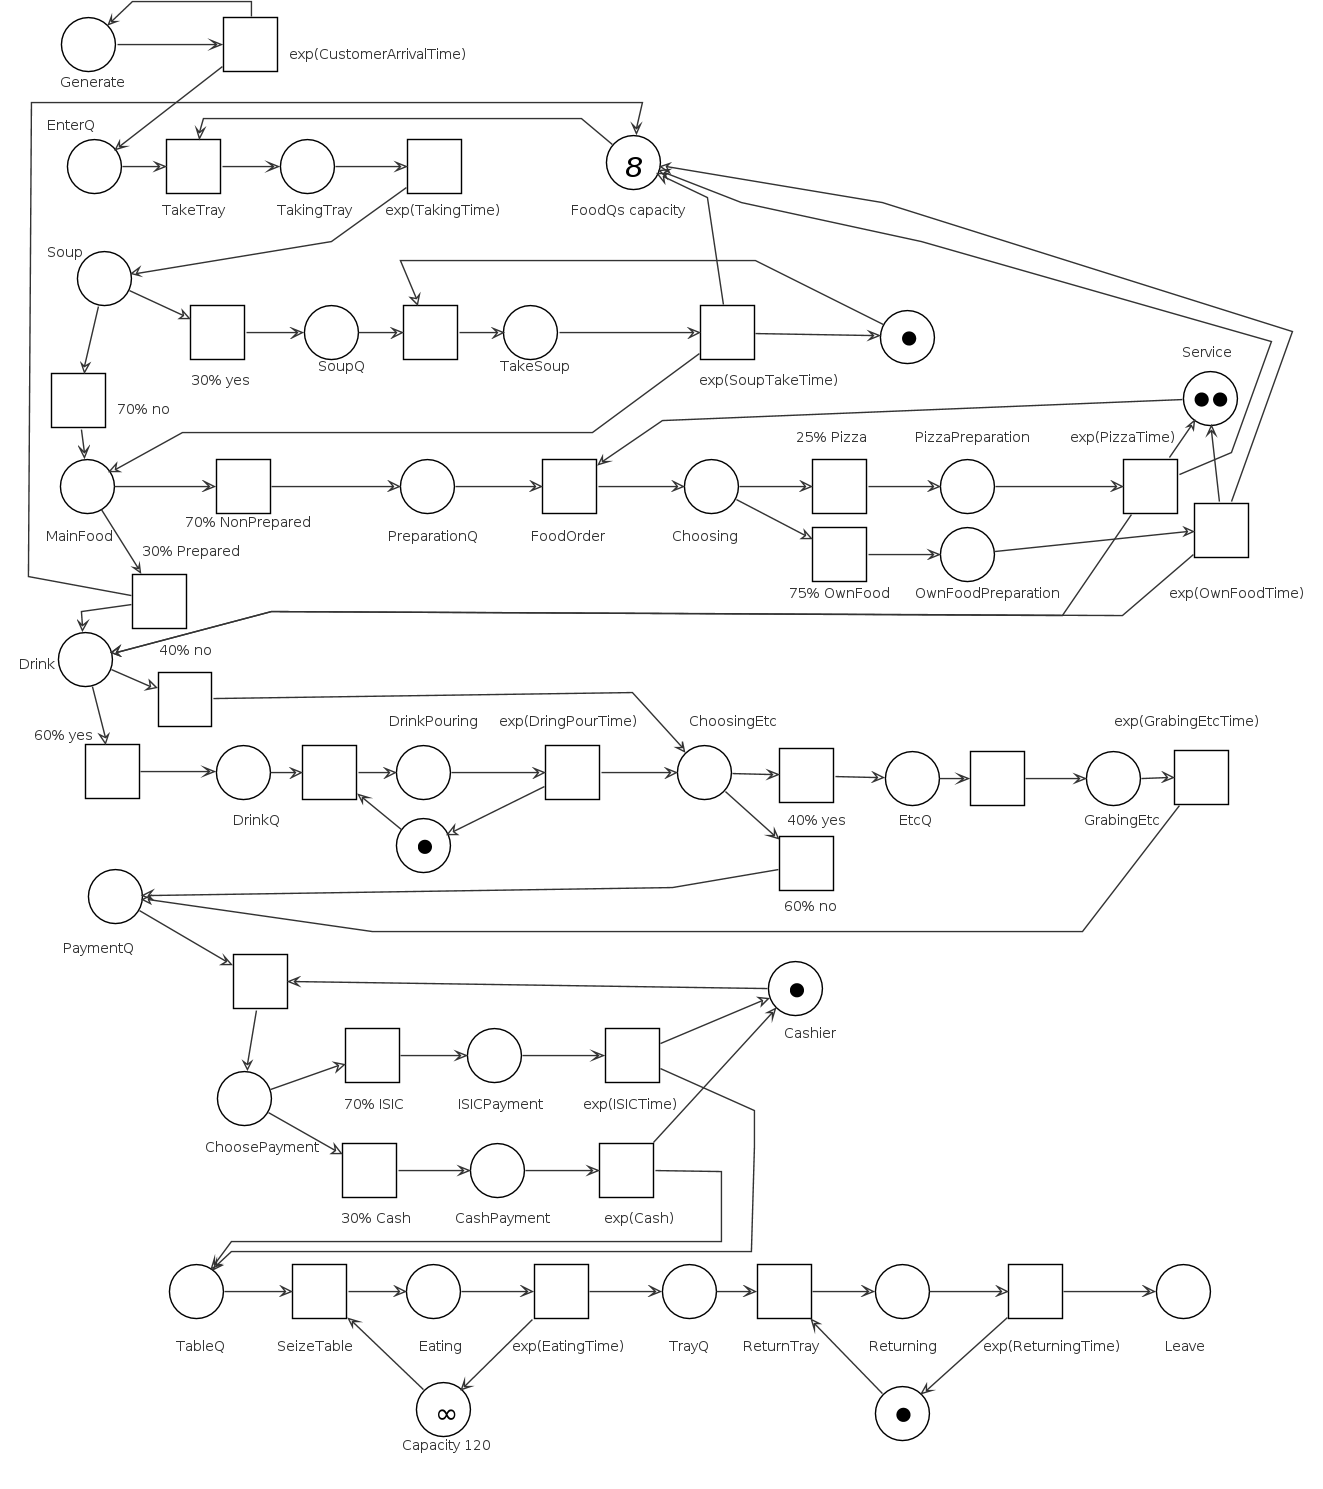
\includegraphics[width=\textwidth,height=16cm,keepaspectratio]{petri_net_menza.png}
  \caption{Petriho sieť: Menza}
  \label{fig:petri_net_canteen}
\end{figure}

\section{Architektúra simulačného modelu}
Implementácia modelu prebehla pomocou jazyka C++ a knižnice Simlib. Boli použité základné komponenty knižnice Simlib a štandardné knižnice jazyka C++.

\subsection{Mapovanie abstaktného modelu na simulačný}
Simulácia sa začína inicializáciou hlavného objektu simulácie - Simulation. Táto simulácia je inicializovaná metódou \texttt{Reinitialize} na základe simulačných dát, ktoré sú jej predané. Simulačné dáta obsahujú dĺžku simulácie a všetky potrebné premenné hodnoty, ktoré sú v simulácii použité. Samotná simulácia je spustená metódou \texttt{Start} na objekte samotnej simulácie. Metóda znova inicializuje všetky potrebné linky k simulácii, čo umožňuje spustenie tej istej simulácie viacnásobne, bez povinnosti znova spúšťať celý program.

Na začiatku simulácie je vytvorený generátor zákazníkov, ktorý prichádzajú do menzy. Tento generátor vytvára udalosti príchodu zákazníkov. Na strane zákazníka sa hneď po vygenerovaní kontroluje dĺžka rady, pričom sa zákazník rozhoduje, či menzu opustí, ak je rada príliš veĺká. V opačnom prípade pokračuje do rady na tácky. Toto je realizované pomocou metódy \texttt{HandleTrayStand}. Ak je stojan na tácky používaný, zákazník sa zaradí do rady a čaká na uvoľnenie stojanu. Ďalšou metódou v rade je \texttt{HandleFood}. Táto metóda rozhoduje o tom, či človek prejde priamo k výberu hlavného jedla, alebo pokračuje do rady na polievku.

Linka výdaja polievky je realizovaná metódou \texttt{HandleSoup}. Ak je linka vólna, zákazníci pristupujú priamo k linke, berú polievku a pokračujú na výber hlavného jedla. V prípade že je linka zrovna zabratá, zákazníci sú vložený do rady, v ktorej čakajú na prístup k linke.

Linka výdaja hlavného jedla je Skladom s kapacitou dva. Táto kapacita predstavuje dvoch zamestnancov, ktorý sa starajú o výdaj hlavného jedla. Podobne ako u linky na polievku, ak je k dispozícii kapacita linky, zákazníci pristupujú priamo k nej, v opačnom prípade sú radený do rady na hlavné jedlo.

Postup obsádzania linky pri jej voľnosti (určuje sa pomocou metódy \texttt{Busy} na linke) je na všetkých linkách taký istý. Ak je linka vóľna, je automaticky obsadená prichádzajúcim zákazníkom, v opačnom prípade je zákazník zaradený do rady danej linky. Toto platí pre ďalšie použité linky na vodu, pochutiny a platobnú linku. Zákazník odchádza zo zariadenia pomocou metódy \texttt{HandleLeave}.

\section{Podstata simulačných experimentov a ich priebeh}
Simulácia má za úlohu zistiť priemerné časy čakania na jednotlivé linky v rôznych časových úsekoch, v ktorých menzy pracujú. Tieto informácie môžu byť ďalej po dobrom uvážení použité na zkvalitnenie procesov v menzách. Vo výsledku by na základe simulácie mal byť navrhnuté zlepšenie menzy tak, aby sa zmenšila čakacia doba zákazníkov a tým sa zvýšil komfort.

\subsection{Postup experimentovania}
Simulácia bola postupne spúšťaná na štyroch rôznych experimentoch, kedy sa menza nachádzala v čase buď pri otvorení, v špičke, v kľudnom chode alebo pred zavretím. Vo všetkých experimentoch boli použité hodnoty namerané priamo v časovom úseku. Stredná hodnota exponenciálnej pravdepodobnosti príchodu zákazníka do menzy bola určená na približne 17 sekúnd. Pri experimentoch bola počítaná celková priepustnosť menzy, respektíve koľko ľudí stihlo menzu opustiť za daný čas. Experimenty boli vždy spúšťané na merítku dvoch hodín, pre lepšie výsledky testov. Výsledky experimentu potom hovoria o presnejšej mierke času, na ktorý boli tieto dve hodiny namapované.

\subsection{Dokumentácia jednotlivých experimentov}
Priepustnosť menzy je v časovom úseku troch hodín približne 600-900 zákazníkov. Vo výsledku typického experimentu, respektíve experimentu s priemernými nameranými hodnotami celkovo, by mala byť táto priepustnosť dodržaná. Experimenty tiež určujú predpoklad priepusntosti menzy v rôznych náporoch.

\subsubsection{Výsledky experimentu pri otvorení}
Experiment prevádzaný v začiatočnom čase otvorenia menzy má stretnú hodnotu funkcie exponenciálnej pravdepodobnosti XXX sekúnd. Začiatočný nápor zákazníkov na menzu je pripočítaný k celkovému priemeru.

\begin{figure}[h!]
  \centering
  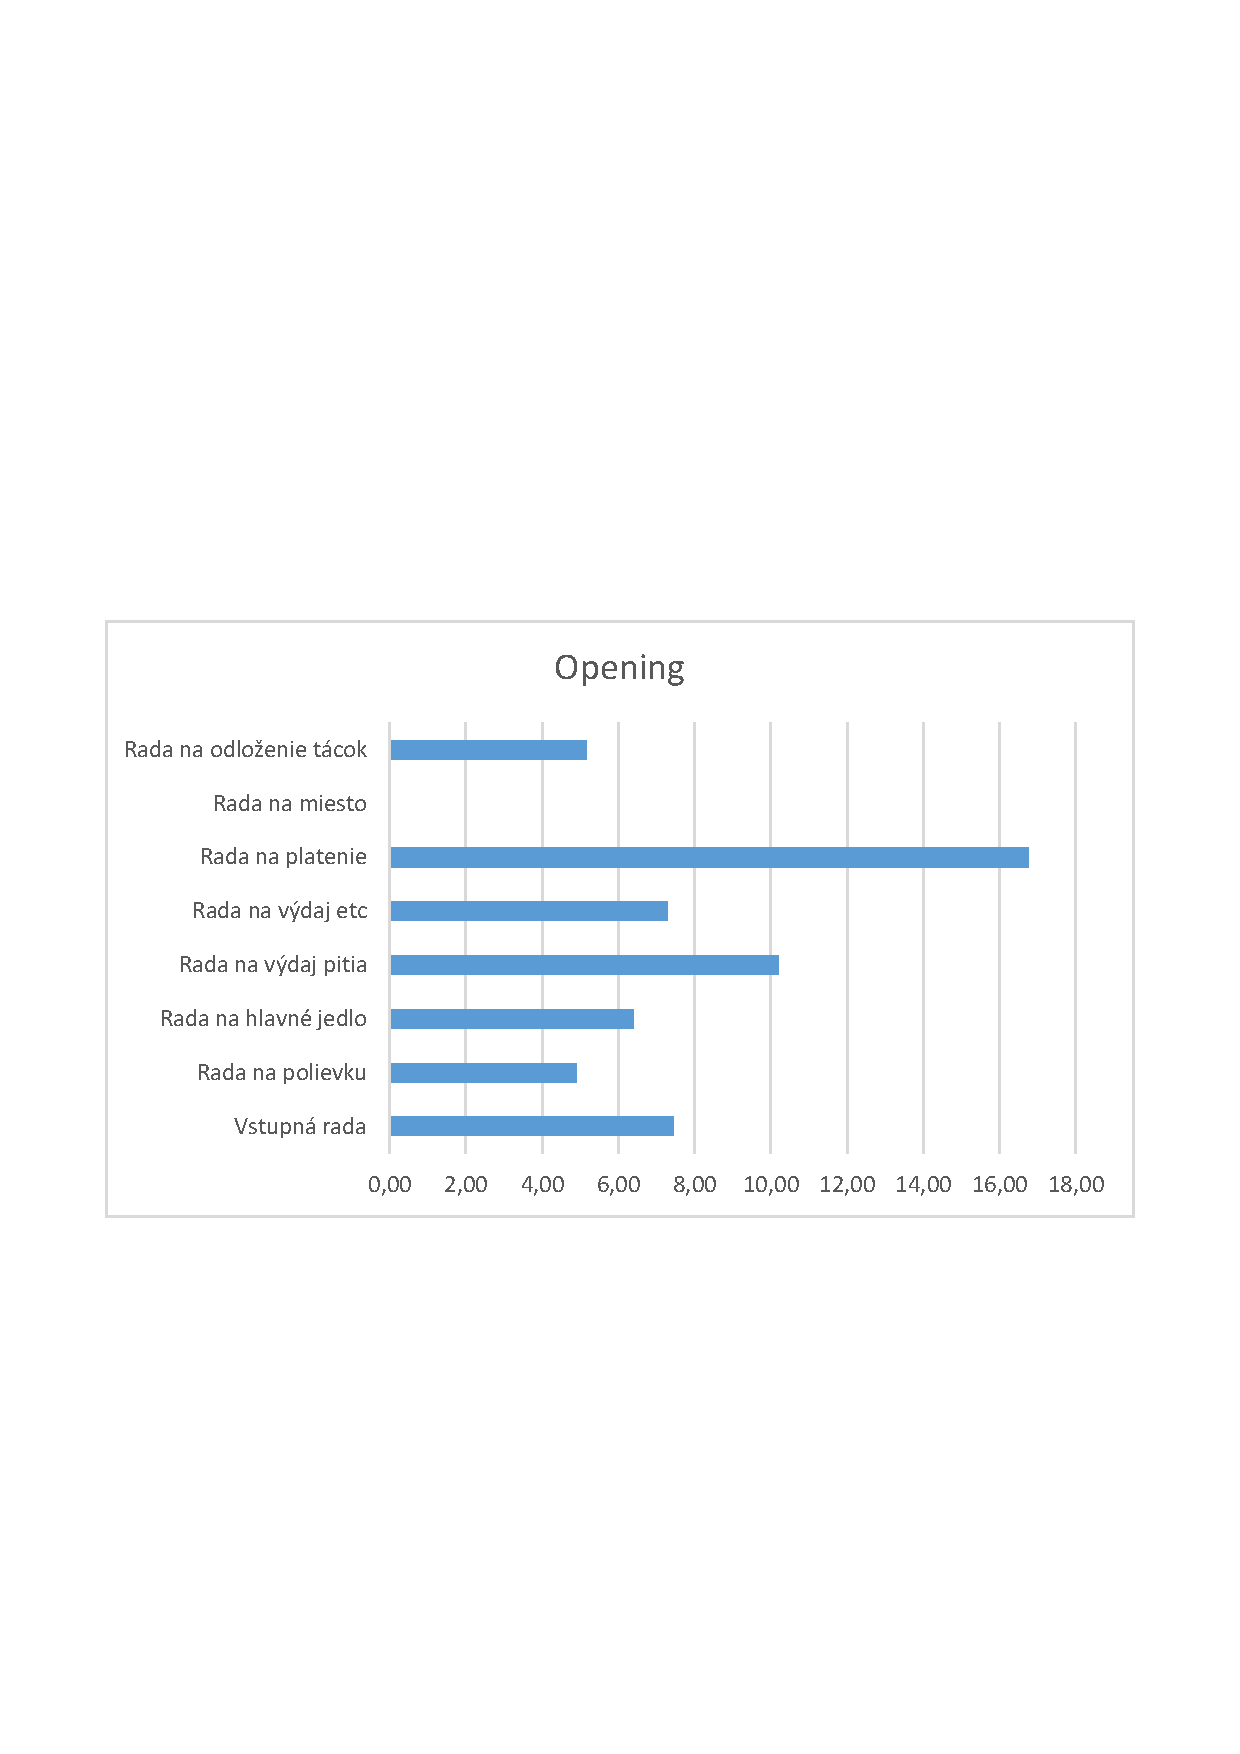
\includegraphics[width=0.8\textwidth,keepaspectratio]{experiment_1.pdf}
  \caption{Maximálne doby čakania na jednotlivé linky}
  \label{fig:experiment_1}
\end{figure}

V experimente je vidieť, že menza v tomto bode zvláda nápor zákazníkov. Čakacie doby na jednotlivé linky nie sú veľké. Čakacie doby neprekročili 20 sekúnd a rada na usadenie sa vôbec nevytvorila.

\pagebreak
\subsubsection{Výsledky experimentu v špičke}
Interval medzi príchodmi zákazníkov je malý, čo je možné vidieť na grafe. Rada pri usádzaní sa vytvára, keďže ľudia majú tendenciu svoje miesto hľadať, platenie teda nie je obmedzené radou na usadenie.

\begin{figure}[h!]
  \centering
  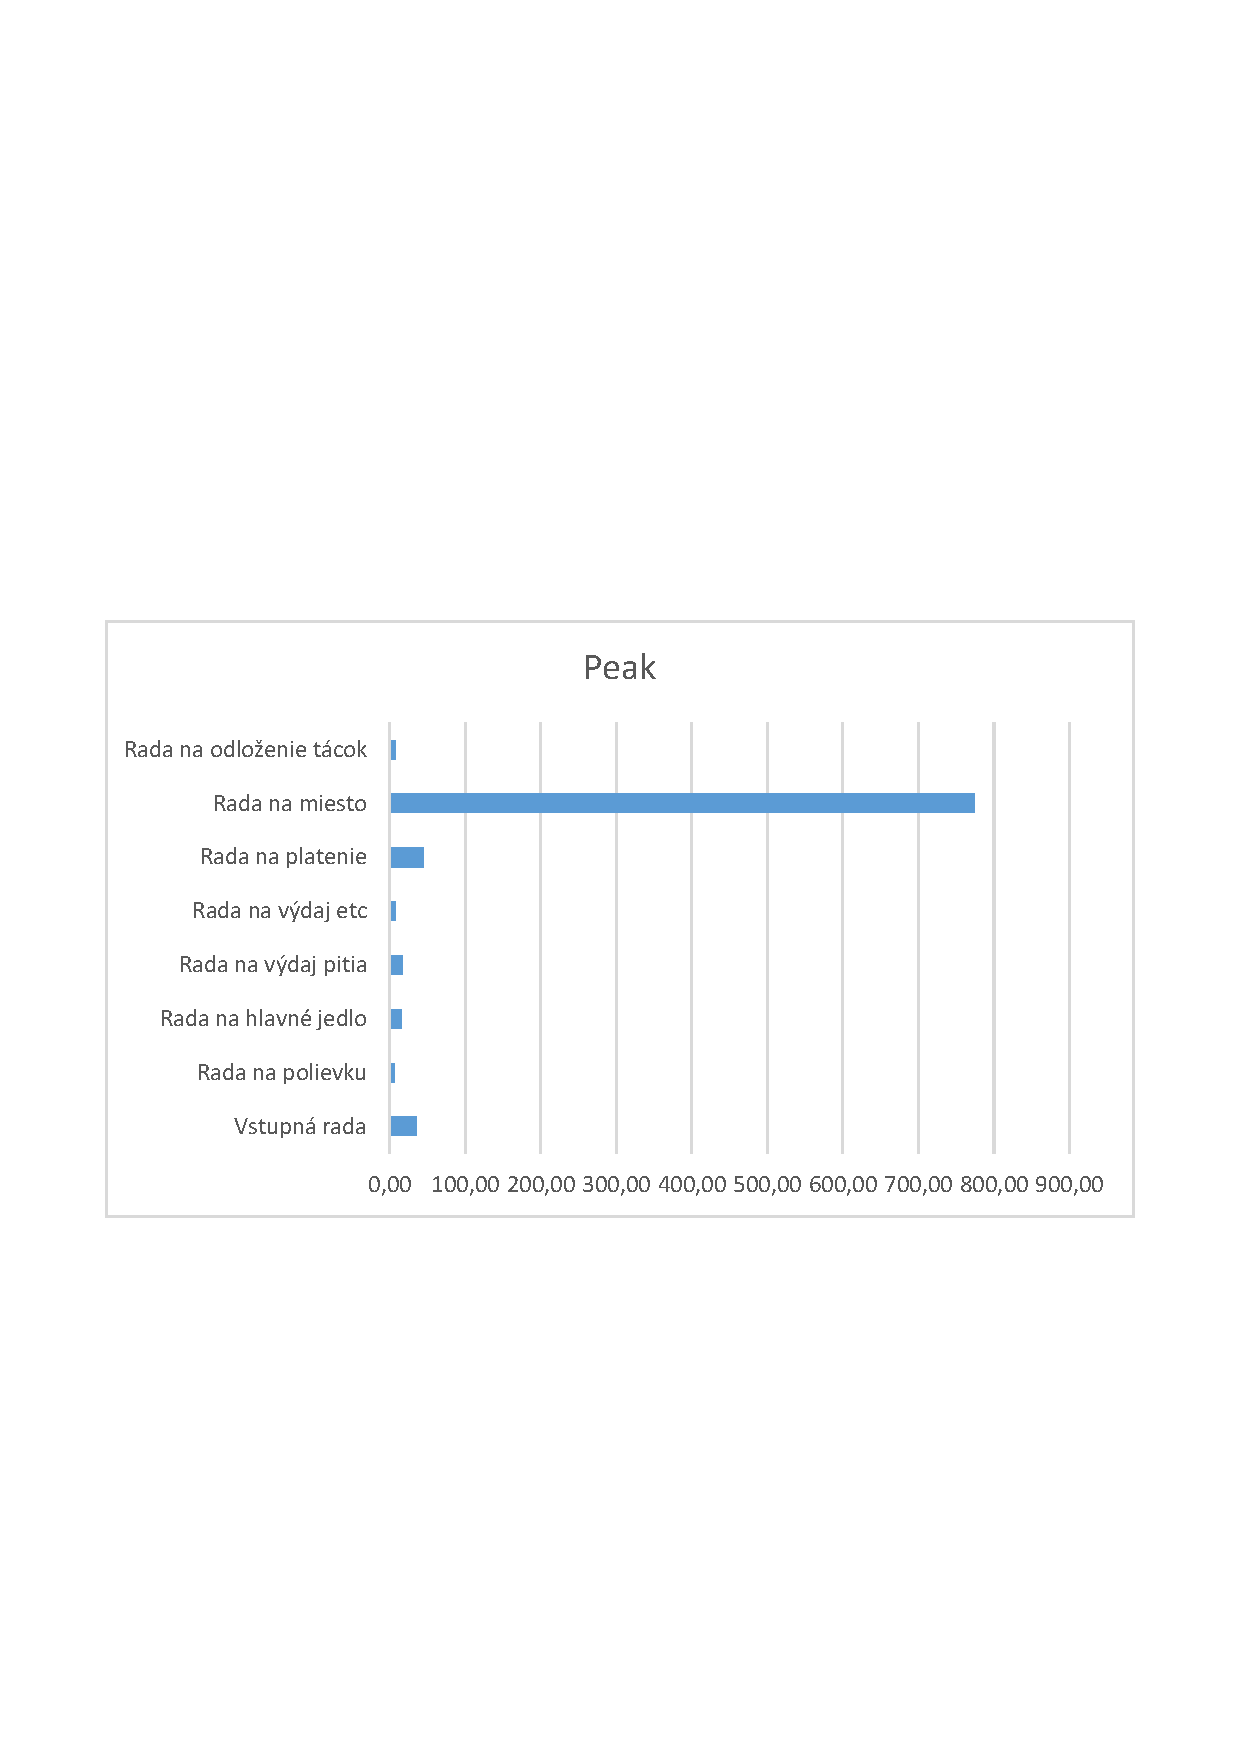
\includegraphics[width=0.8\textwidth,keepaspectratio]{experiment_2.pdf}
  \caption{Maximálne doby čakania na jednotlivé linky}
  \label{fig:experiment_2}
\end{figure}

V grafe je možnosť všimnúť si vysokú čakaciu dobu na usadenie. Toto je spôsobené simulovaním špičky v rámci dvoch hodín, aj v nižších časoch sa však stáva, že zákazník musí na miesto pri stole čakať. V tomto prípade je teda jasné, že optimalizácia stravovacieho zariadenia by spočívala práve v rozšírení kapacít, ktoré menza poskytuje na usadenie.

\pagebreak
\subsubsection{Výsledky experimentu v kľude}
Experiment prebieha v čase kedy je množstvo prichádzajúcich zákazníkov stály a čas mezdi príchodmi relatívne veľký. Zákazníci majú možnosť sa bez problémov usadiť.


\begin{figure}[h!]
  \centering
  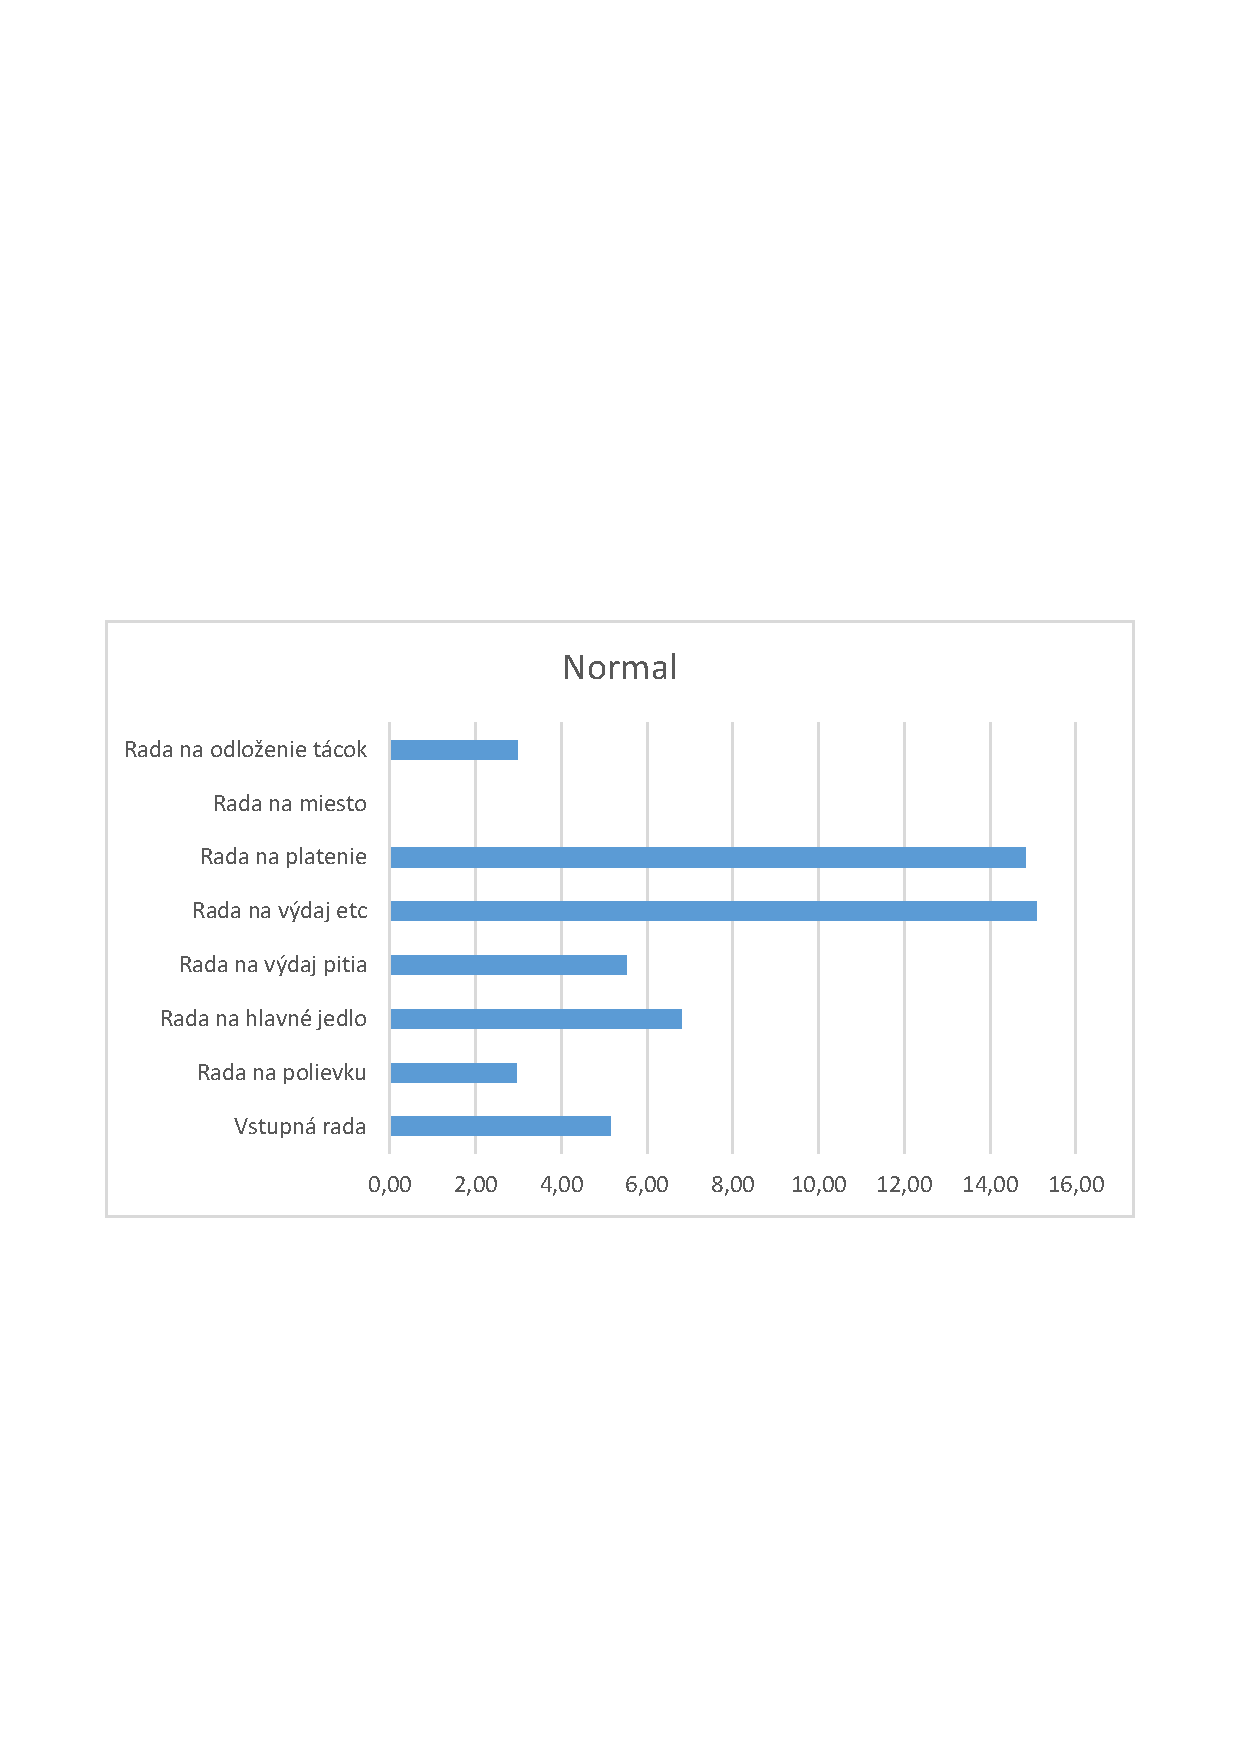
\includegraphics[width=0.8\textwidth,keepaspectratio]{experiment_3.pdf}
  \caption{Maximálne doby čakania na jednotlivé linky}
  \label{fig:experiment_3}
\end{figure}


Tento stav menza zažíva medzi jednotlivími stavmi náporu a môžeme na ňom pozorovať, že má tendenciu vyrovnávať zvýšené počty ľudí v radách naspäť do prijateľných stavov.

\pagebreak
\subsubsection{Výsledky experimentu pri zatváraní}
Výsledky experimentu sú podobné ako výsledky pri otváraní, keďže bol pri zatváraní stravovacieho zariadenia zaznamenaný podobný počet príchodov ako pri otváraní. Toto je spôsobené koncami prednášok v tomto čase. Pri uzatváraní menzy hovoríme o miernej špičke, ktorá nárazovo zvyšuje počet príchodov.

\begin{figure}[h!]
  \centering
  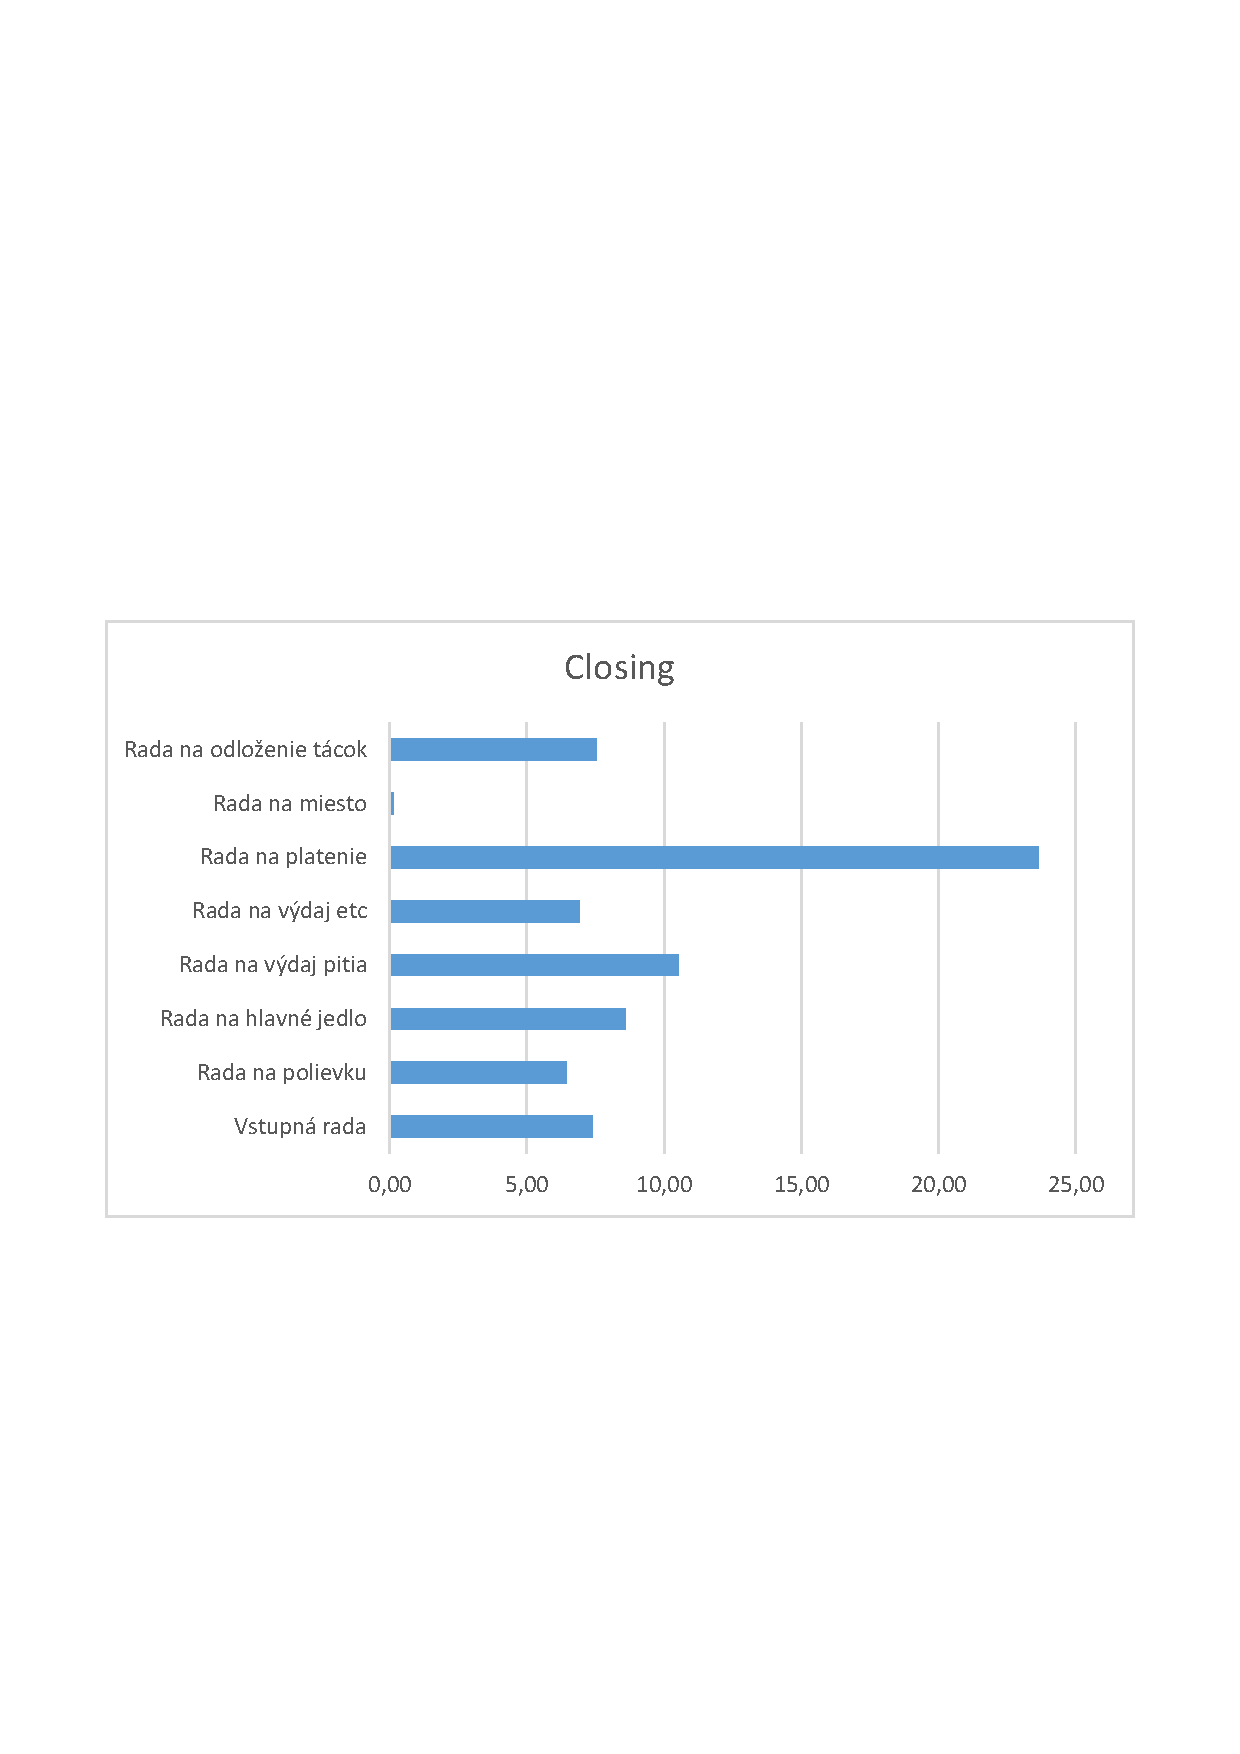
\includegraphics[width=0.8\textwidth,keepaspectratio]{experiment_4.pdf}
  \caption{Maximálne doby čakania na jednotlivé linky}
  \label{fig:experiment_4}
\end{figure}

Vďaka zvýšenému náporu zákazníkov v čase pred zatvorením menzy sú vytvorené menšie rady pri všetkých linkách. Toto však neovplyvňuje linku usadenia zákazníka. Ľudia teda stíhajú odchádzať skôr, ako stíhajú prichádzať nový.

\subsection{Závery experimentov}
Všetky štyry experimenty, ktoré boli simulované, určujú fungovanie menzy v rôznych bodoch, ako bolo diskutované na začiatku. Experimenty pri otvorení a zatvorení menzy sú veľmi podobné, keďže dáta ukazujú, že na menzu je takmer taký istý nápor zákazníkov.

\section{Zhrnutie simulačných experimentov a záver}
Testovacím programom \texttt{typical} bola overená funkčnosť modelu. Na základe toho boli potom určené 4 experimenty, ktoré sa zameriavali na rôzne časové úseky fungovania menzy. Experimenty ukazujú zvýšenú náročnosť a čakanie v radách v časoch, kedy je vstup zákazníkov do menzy veľký.

Experimenty je možné ďalej upravovať a odhaliť tak ďalšie slabé miesta fungovania menzy. Jedným zo slabých miest je práve platobná kasa. Pre zlepšenie priepustnosti zákazníkov cez zariadenie v čase špičky je teda vhodné umiestniť viac platobných kás, aby sa predišlo čakaniu, kedy kedy je výdaj jedla schopný túto radu zasýtiť. Tiež je vhodné zväčšiť kapacitu menzy pre zákazníkov.

\pagebreak

  \begin{thebibliography}{1}

  \bibitem{ims}
  \href{http://www.fit.vutbr.cz/study/courses/IMS/public/prednasky/IMS.pdf}{IMS Slajdy} \newline
  \href{http://www.fit.vutbr.cz/study/courses/IMS/public/prednasky/IMS.pdf}{\nolinkurl{http://www.fit.vutbr.cz/study/courses/IMS/public/prednasky/IMS.pdf}}
  
  \bibitem{menzy}
  \href{http://www.kam.vutbr.cz/?p=nabs}{Informácie o menzách} \newline
  \href{http://www.kam.vutbr.cz/?p=nabs}{\nolinkurl{http://www.kam.vutbr.cz/?p=nabs}}
  
  \bibitem{simlib}
  \href{http://www.fit.vutbr.cz/~peringer/SIMLIB/}{Simlib} \newline
  \href{http://www.fit.vutbr.cz/~peringer/SIMLIB/}{\nolinkurl{http://www.fit.vutbr.cz/~peringer/SIMLIB/}}
  
  \bibitem{examples}
  \href{http://www.fit.vutbr.cz/~peringer/SIMLIB/examples/}{Simlib} \newline
  \href{http://www.fit.vutbr.cz/~peringer/SIMLIB/examples/}{\nolinkurl{http://www.fit.vutbr.cz/~peringer/SIMLIB/examples}}

  \end{thebibliography}

\end{document}
